We compare the performance of LP-RFFs with full-precision RFFs (FP-RFFs), circulant FP-RFFs, and the \Nystrom method, on the TIMIT, YearPred, CovType, and Census datasets, showing that we can attain compression ratios of at least 2.4x relative to these methods, without hurting generalization performance. We then perform a more careful analysis of these results on the Census dataset and a sub-sampled version of the CovType dataset, where we plot the generalization performance of these approximation methods relative to their relative spectral distances. We observe on both datasets that the relative spectral distance appears much more predictive of generalization performance than more standard metrics like the Frobenius and spectral norms of $K-\tK$. Finally, we show that we can perform all model updates in low-precision using a recently proposed low-precision training algorithm called LM-HALP (linear model high accuracy low precision) \citep{halp18}.

For all our experiments, we use the Gaussian kernel with the kernel width value recommended by~\citet{may2017}, and compute the memory utilization as described in Section~\ref{subsec:memory_utils}. To evaluate the performance of these kernel models, we measure the classification error for classification tasks, and the mean squared error (MSE) for regression tasks ($\frac{1}{n}\sum_{i=1}^n (f_{\tK}(x_i) - y_i)^2$), on the heldout set. We note that in our experiments, in order to avoid the risk of numerical precision issues (kernel ridge regression requires matrix inversion), we do all our full-precision experiments in 64 bits.  Nonetheless, we calculate the memory utilization of these experiments as if we used 32 bits, to avoid inflating the relative gains of our method over the full-precision approaches.  We include more details about our datasets, experimental protocols, and hyperparameter choices in Appendix~\ref{subsec:app_exp_detail}.\vsp

\subsection{Empirical evaluation of LP-RFFs}
\label{sec:full_run}
We compare the generalization performance of LP-RFFs to FP-RFFs, circulant FP-RFFs, and \Nystrom features, across four datasets, for various memory budgets.  We sweep the following hyperparameters: For LP-RFFs, we choose the precision $b \in \{1,2,4,8,16\}$. For \NystromNS, we use $m \in \{1250, 2500, 5000, 10000, 20000\}$.  For the RFF-based methods, we use $m\in \{1250, 2500, 5000, 10000, 20000, 50000, 100000, 200000, 400000\}$. We choose these limits differently because $\num[group-separator={,}]{20000}$ \Nystrom features have roughly the same memory footprint as $\num[group-separator={,}]{400000}$ FP-RFFs. For all experiments, we use a mini-batch size of $250$.  We use an automatic early-stopping protocol, as in \citep{morgan1990generalization,sainath2013b,sainath2013low}, in order to regularize our models \citep{zhang2005boosting,wei2017early} and avoid expensive hyperparameter tuning (for details see Appendix~\ref{subsec:app_exp_detail}).

In Figure \ref{fig:generalization_col}, we plot the generalization performance for these experiments, as a function of the amount of total memory used (all 3 components in Table~\ref{table:mem-usage}), for TIMIT, YearPred, and CovType. LP-RFFs show better generalization performance than the full-precision baselines under various memory budgets. For clarity, we only plot LP-RFF results for 4 and 8 bits. To see results for all precisions, as well as for plots showing performance as a function of the number of features, and for Census results, see Appendix~\ref{subsec:app_additional_exp_res}. Here, we see that similar to \citet{nysvsrff12}, the \Nystrom method has better generalization performance than the RFF-based methods with the same number of features. However, when we instead consider performance as a function of memory utilization, the opposite it true, with the RFF-based methods demonstrating superior generalization performance. We also see that LP-RFFs (which use circulant projections) also significantly outperform circulant FP-RFFs, showing that the performance improvement under memory budget comes primarily from using low-precision features.

In Table~\ref{tab:mem_saving} we present the compression ratios we achieve with LP-RFFs, relative to the baseline methods, while still attaining generalization performance within $10^{-4}$ of the full-precision baseline.  We measure this as follows: For each baseline (FP-RFFs, circulant FP-RFFs, \NystromNS), we find the best performing model. We then find the smallest LP-RFF model, as well as the smallest baseline model, which attains within $10^{-4}$ relative performance to the best performing baseline. We report the ratio of the memory used by these two models (baseline/LP-RFF), that are both within $10^{-4}$ of the best baseline. We compute this ratio across three independent runs using different random seeds, and report the average.  We can see that LP-RFFs demonstrate significant memory saving over FP-RFFs, circulant FP-RFFs, and \NystromNS, showing 2.9x-10.3x, 2.4x-15.6x, and 50.9x-461.6x compression ratios respectively. On the TIMIT dataset, there are 147 classes, and thus the full-precision learned parameters occupy a large portion of the total memory across all methods. Nonetheless, even though these LP-RFF experiments only quantize the feature mini-batches, they still attain 5.1x and 2.4x compression ratios relative to FP-RFF and circulant FP-RFF.


\begin{figure}
	\centering
	\begin{small}
	\begin{tabular}{@{\hskip -0.05in}c@{\hskip -0.1in}c@{\hskip -0.1in}c@{\hskip -0.05in}}
		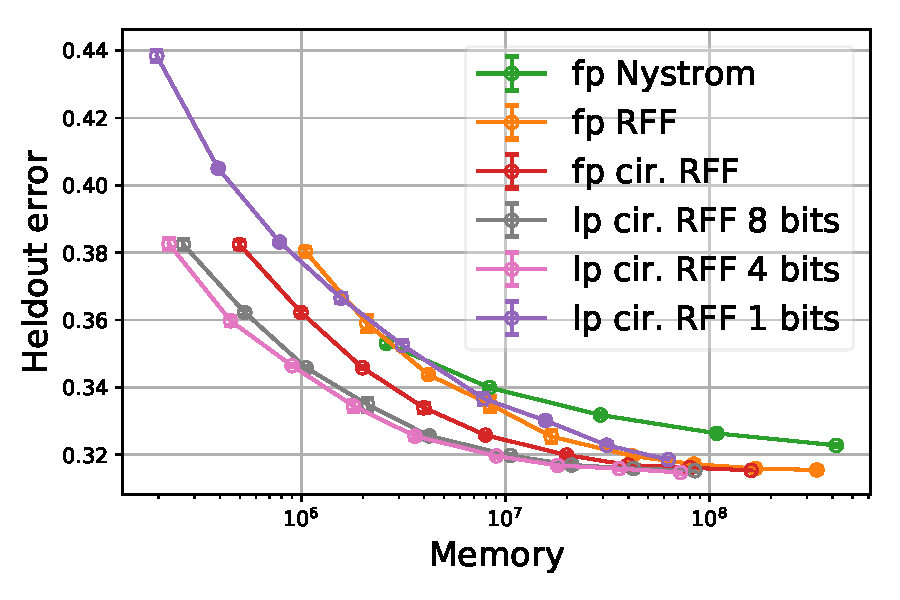
\includegraphics[width=0.34\linewidth]{figures/timit_error_vs_n_memory.pdf} &	
		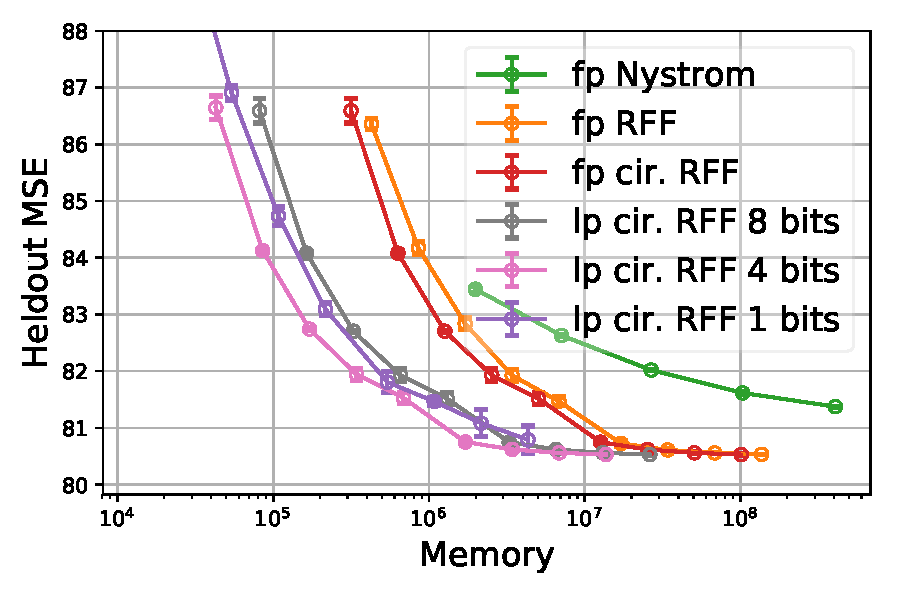
\includegraphics[width=0.34\linewidth]{figures/yearpred_MSE_vs_n_memory.pdf} &
		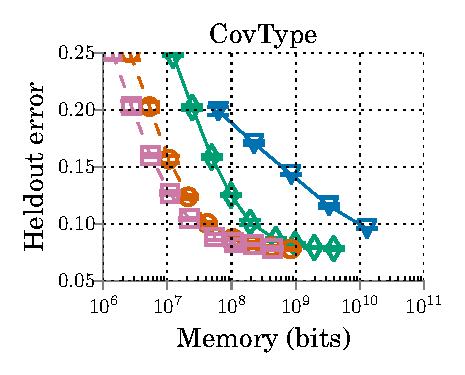
\includegraphics[width=0.34\linewidth]{figures/covtype_error_vs_n_memory.pdf} \vspace{-0.1in}\\
		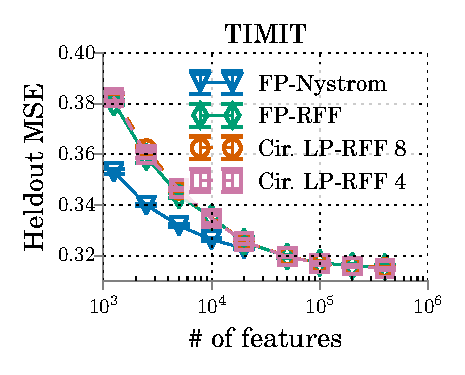
\includegraphics[width=0.34\linewidth]{figures/timit_error_vs_n_feat.pdf} &	
		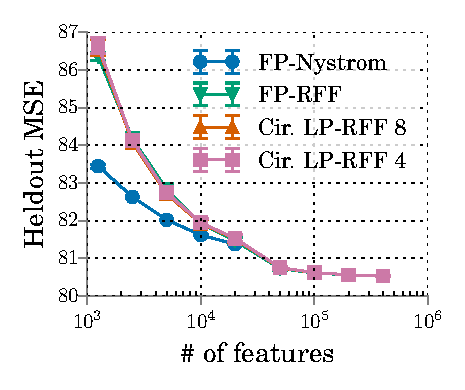
\includegraphics[width=0.34\linewidth]{figures/yearpred_MSE_vs_n_feat.pdf} &
		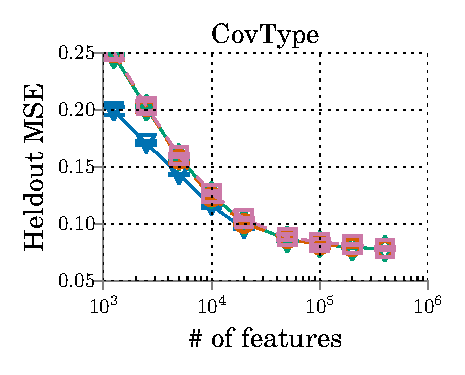
\includegraphics[width=0.34\linewidth]{figures/covtype_error_vs_n_feat.pdf}	
%		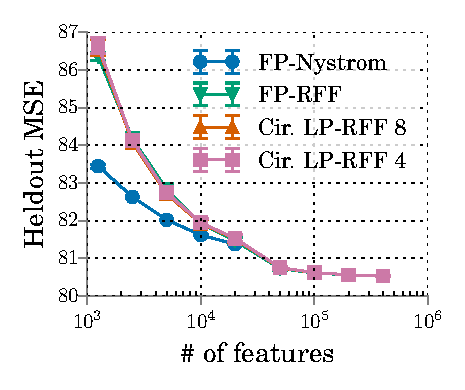
\includegraphics[width=0.26\linewidth]{figures/yearpred_MSE_vs_n_feat.pdf} &	
%		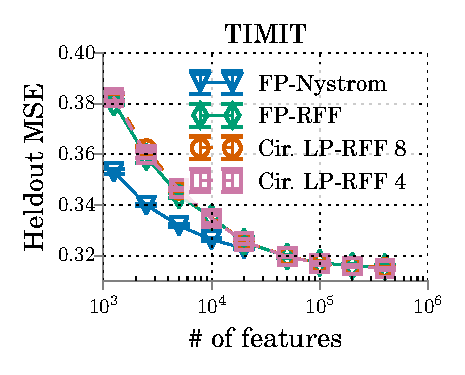
\includegraphics[width=0.26\linewidth]{figures/timit_error_vs_n_feat.pdf} &
%		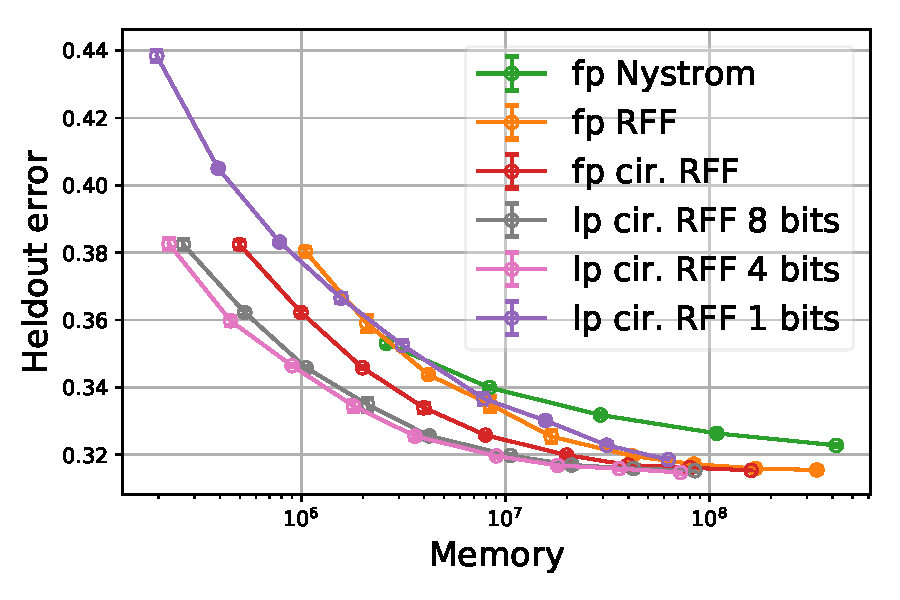
\includegraphics[width=0.26\linewidth]{figures/timit_error_vs_n_memory.pdf} &
%		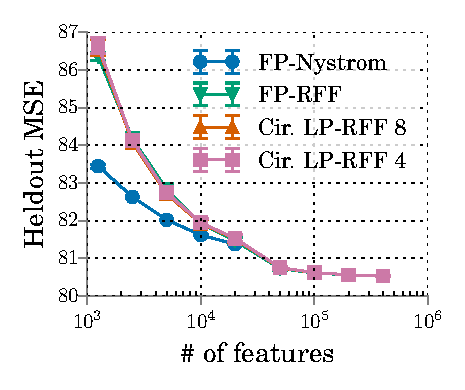
\includegraphics[width=0.26\linewidth]{figures/yearpred_MSE_vs_n_feat.pdf} & 
%		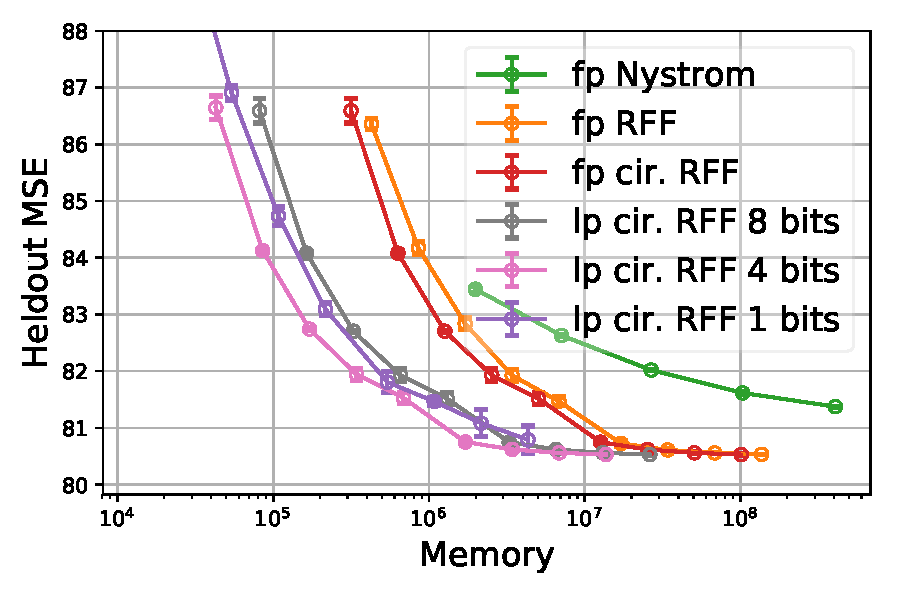
\includegraphics[width=0.26\linewidth]{figures/yearpred_MSE_vs_n_memory.pdf}
%\\
%		(a) TIMIT: Err. vs. Feat. & (b) TIMIT: Err. vs. Mem. & (c) YearPred: MSE vs. Feat. & (d) YearPred: MSE vs. Feat. \\
%		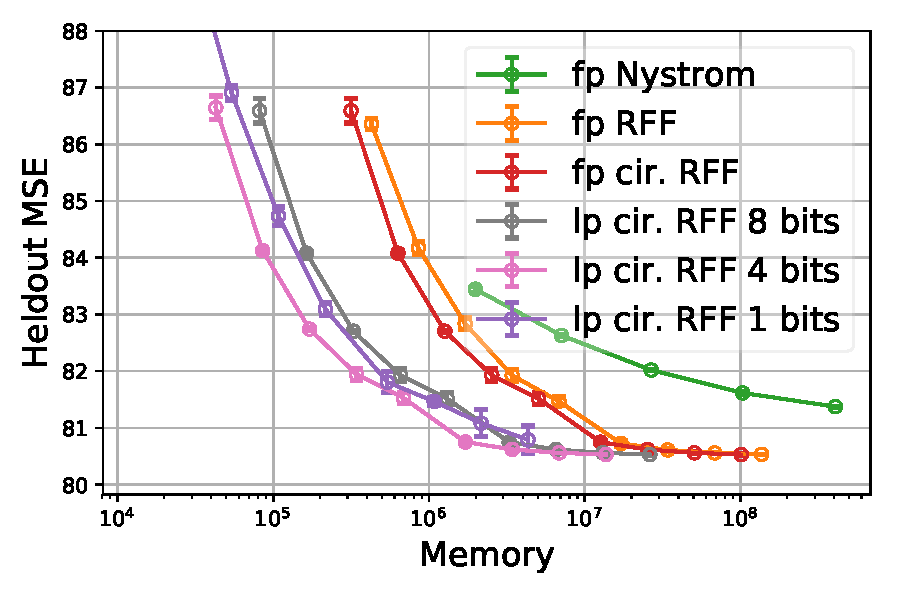
\includegraphics[width=0.3\linewidth]{figures/yearpred_MSE_vs_n_memory.pdf} &
%		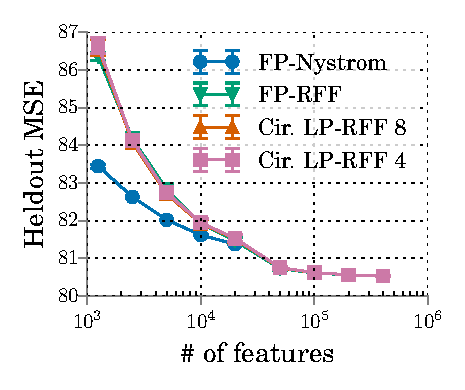
\includegraphics[width=0.3\linewidth]{figures/yearpred_MSE_vs_n_feat.pdf} &
%		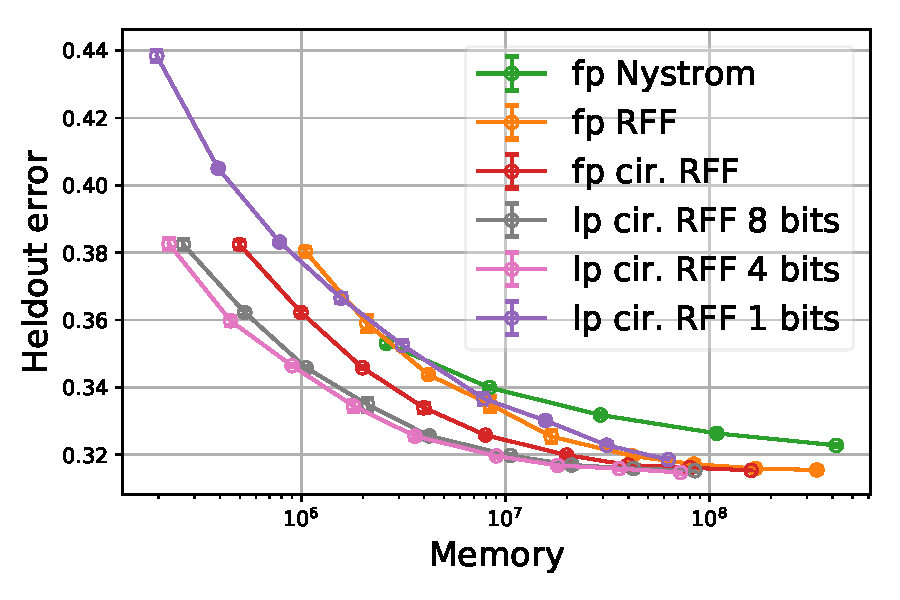
\includegraphics[width=0.3\linewidth]{figures/timit_error_vs_n_memory.pdf} &
%		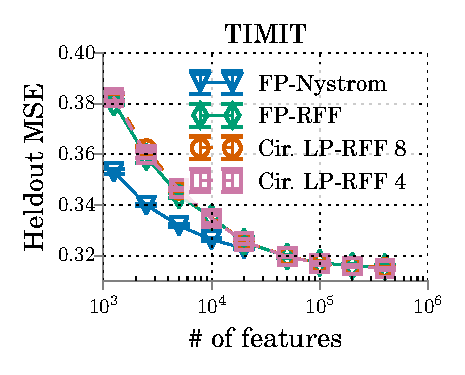
\includegraphics[width=0.3\linewidth]{figures/timit_error_vs_n_feat.pdf} \\
%		(a) Census & (b) YearPred & (c) Covtype & (d) TIMIT \\
%		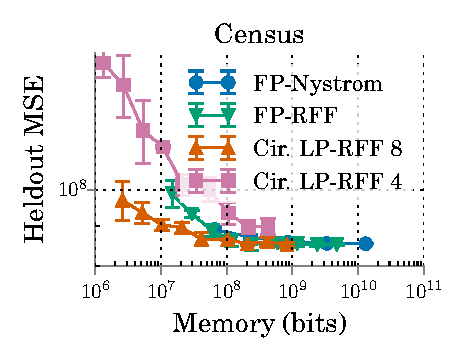
\includegraphics[width=0.3\linewidth]{figures/census_MSE_vs_n_memory.pdf} &
%		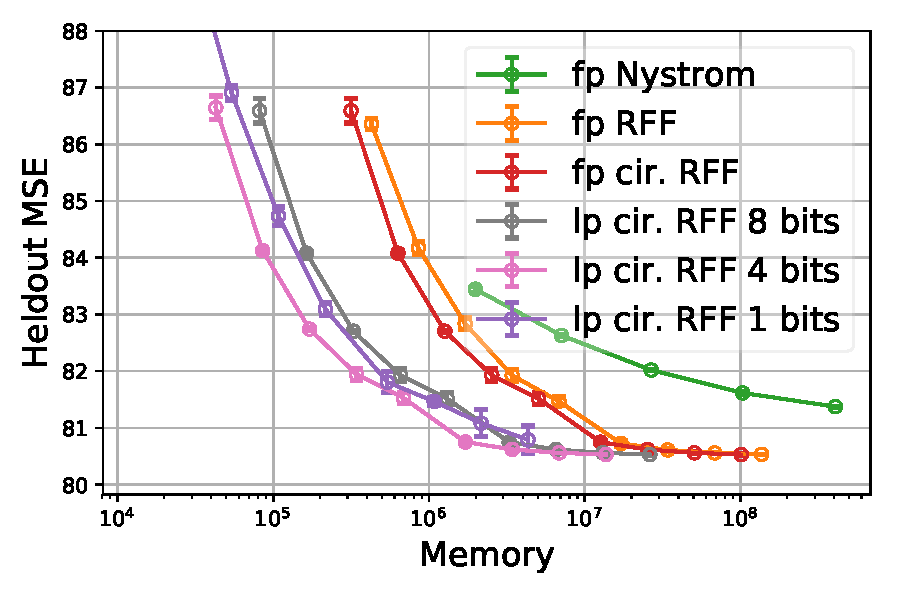
\includegraphics[width=0.3\linewidth]{figures/yearpred_MSE_vs_n_memory.pdf} &
%		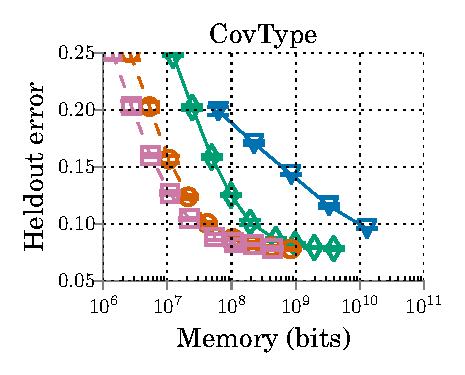
\includegraphics[width=0.3\linewidth]{figures/covtype_error_vs_n_memory.pdf} &
%		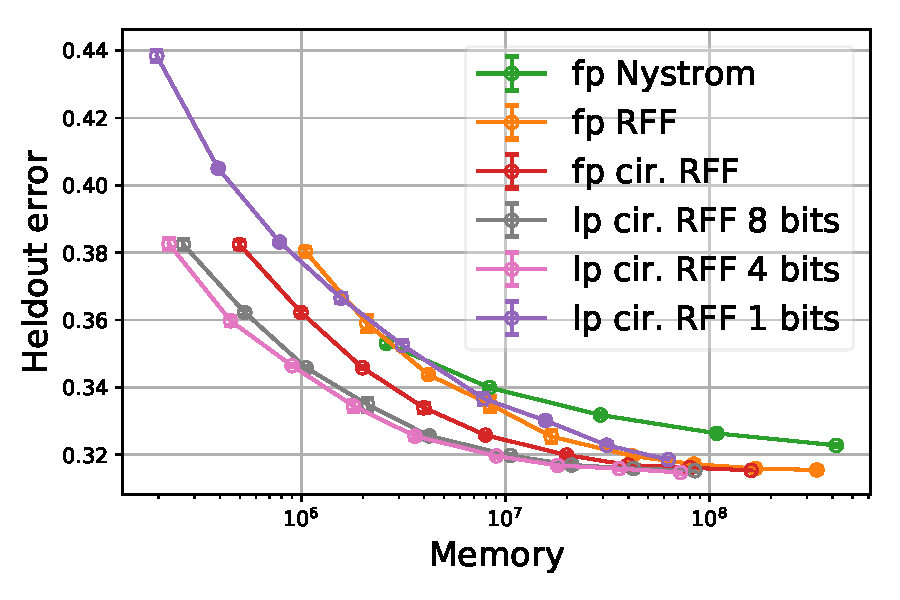
\includegraphics[width=0.3\linewidth]{figures/timit_error_vs_n_memory.pdf} \\
%		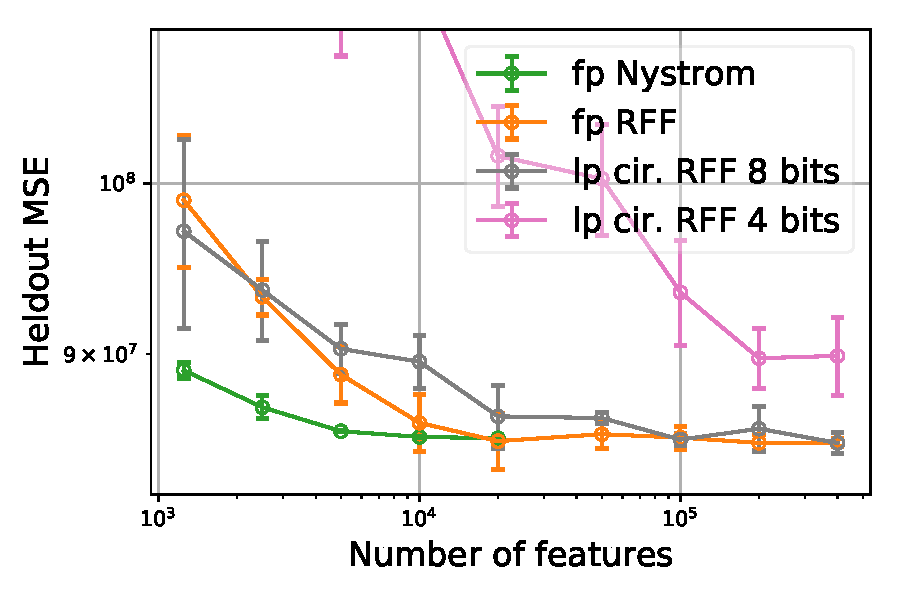
\includegraphics[width=0.3\linewidth]{figures/census_MSE_vs_n_feat.pdf} &
%		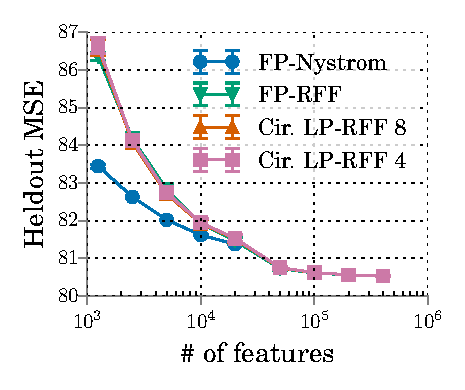
\includegraphics[width=0.3\linewidth]{figures/yearpred_MSE_vs_n_feat.pdf} &
%		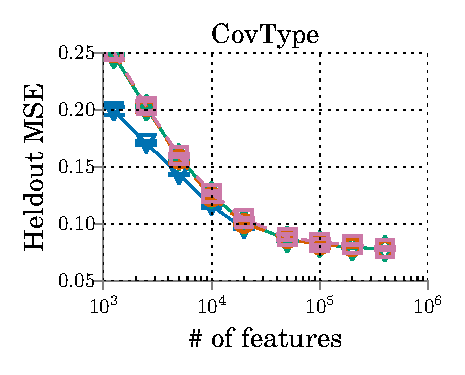
\includegraphics[width=0.3\linewidth]{figures/covtype_error_vs_n_feat.pdf} &
%		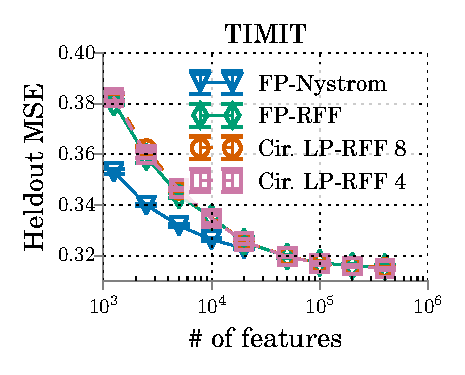
\includegraphics[width=0.3\linewidth]{figures/timit_error_vs_n_feat.pdf} \\
%		(a) Census & (b) YearPred & (c) Covtype & (d) TIMIT \\
	\end{tabular}
	\end{small}
	\caption{Generalization performance of LP-RFFs, FP-RFFs, and \Nystrom with respect to memory, on TIMIT and YearPred and CovType. The same trend holds for Census; see Appendix~\ref{subsec:app_exp_detail}.
		%  LP-RFFs demonstrate better generalization performance than the full precision methods, under a memory budget. It is also informative to observe that while the \Nystrom method attains the best generalization performance with respect to the number of features, it is the worst performance method as a function of memory.  For results on the CovType and Census datasets, please see Figure~\ref{fig:generalization_col_app} in Appendix~\ref{sec:exp_details}
}
	\label{fig:generalization_col}
\end{figure}

%\begin{figure}
%	\centering
%	\begin{small}
%	\begin{tabular}{@{\hskip -0.05in}c@{\hskip -0.1in}c@{\hskip -0.1in}c@{\hskip -0.1in}c@{\hskip -0.05in}}
%%		\subfigure[YearPred MSE vs. Mem.]{\label{fig:year_pred_mem} 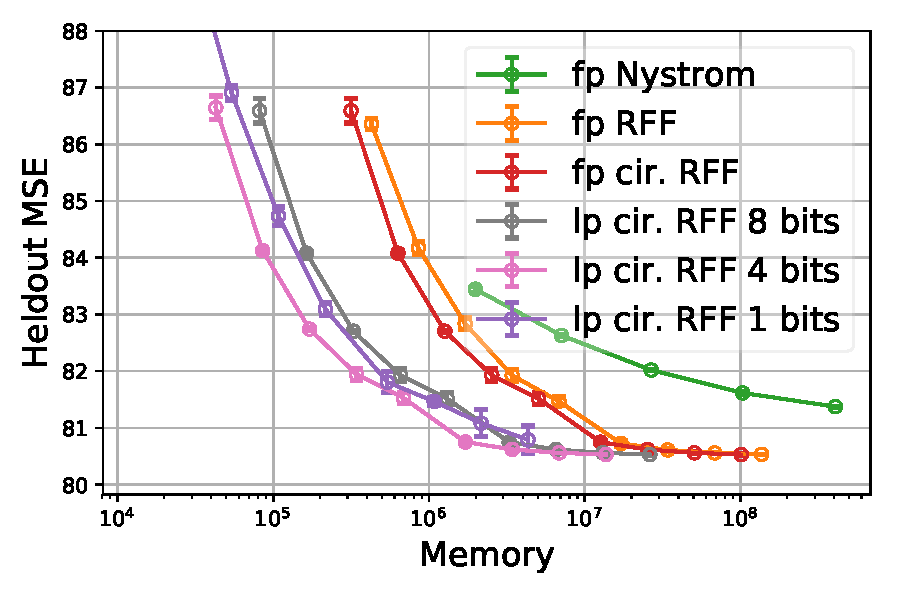
\includegraphics[width=0.27\linewidth]{figures/yearpred_MSE_vs_n_memory.pdf} } \hfill
%%		\subfigure[TIMIT Err. vs. Mem.]{\label{fig:year_pred_mem} 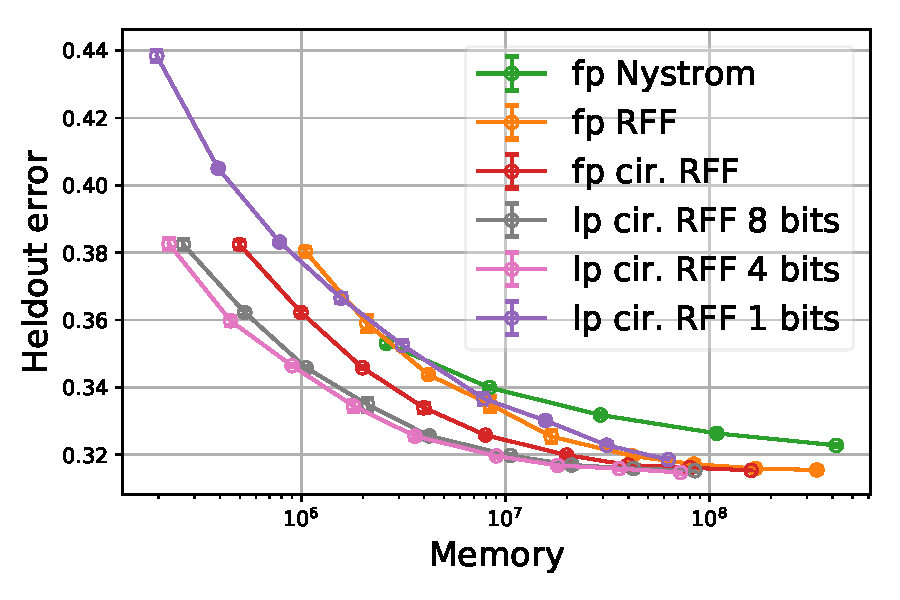
\includegraphics[width=0.27\linewidth]{figures/timit_error_vs_n_memory.pdf} } \hfill
%%		\subfigure[YearPred MSE vs. Feat.]{\label{fig:year_pred_feat}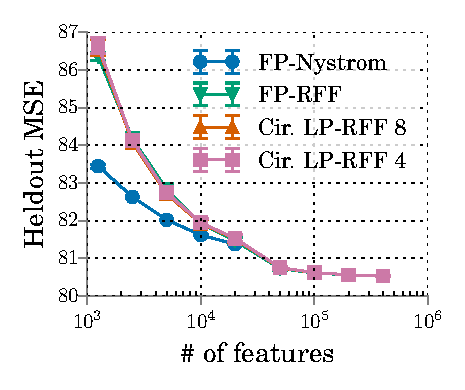
\includegraphics[width=0.27\linewidth]{figures/yearpred_MSE_vs_n_feat.pdf} } \hfill
%%		\subfigure[TIMIT Err vs. Feat.]{\label{fig:year_pred_feat}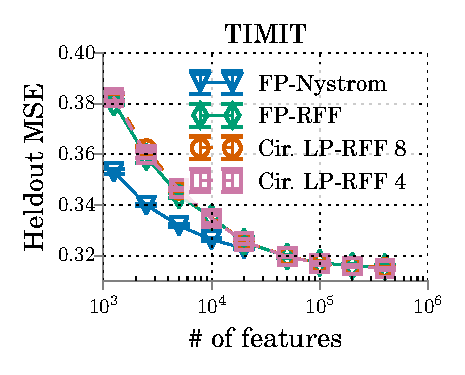
\includegraphics[width=0.27\linewidth]{figures/timit_error_vs_n_feat.pdf} } \hfill
%		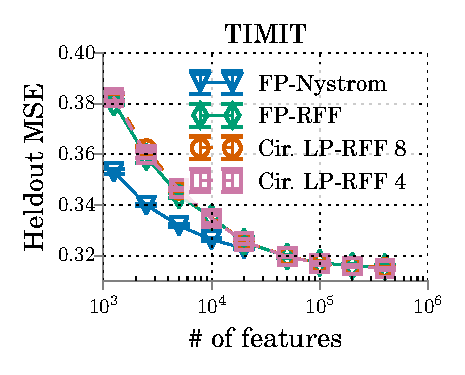
\includegraphics[width=0.26\linewidth]{figures/timit_error_vs_n_feat.pdf} &
%		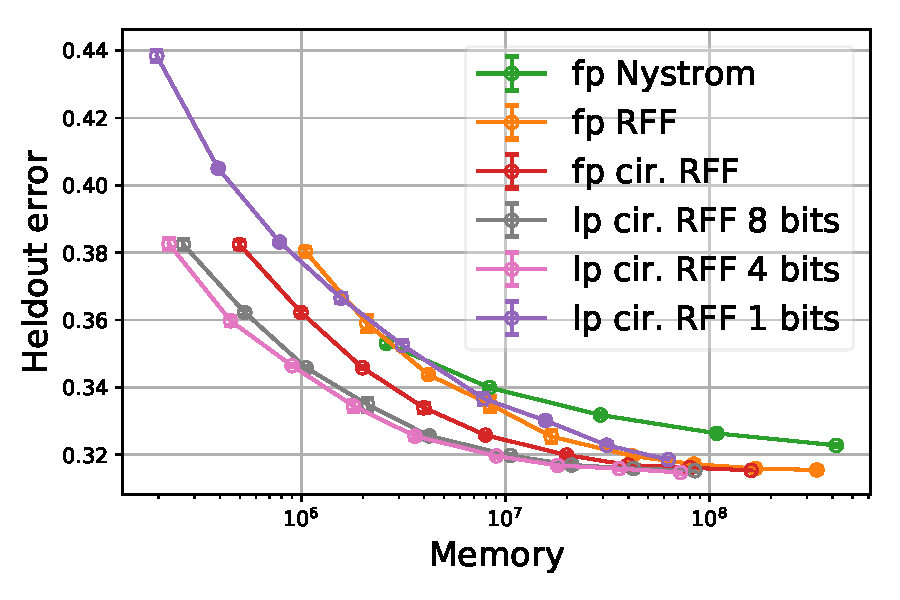
\includegraphics[width=0.26\linewidth]{figures/timit_error_vs_n_memory.pdf} &
%		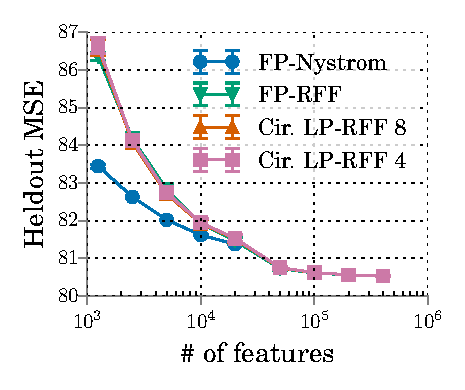
\includegraphics[width=0.26\linewidth]{figures/yearpred_MSE_vs_n_feat.pdf} & 
%		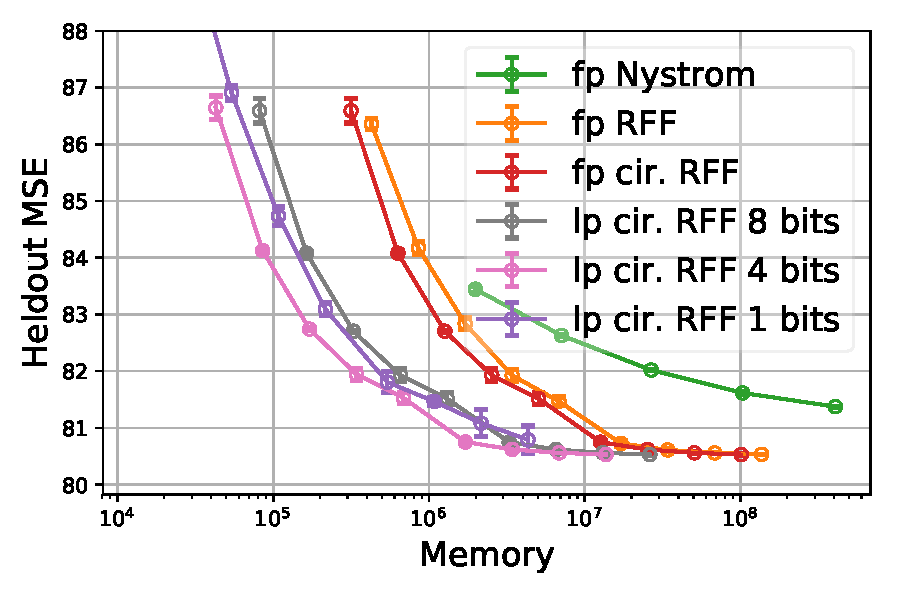
\includegraphics[width=0.26\linewidth]{figures/yearpred_MSE_vs_n_memory.pdf}
%\\
%%		(a) TIMIT: Err. vs. Feat. & (b) TIMIT: Err. vs. Mem. & (c) YearPred: MSE vs. Feat. & (d) YearPred: MSE vs. Feat. \\
%%		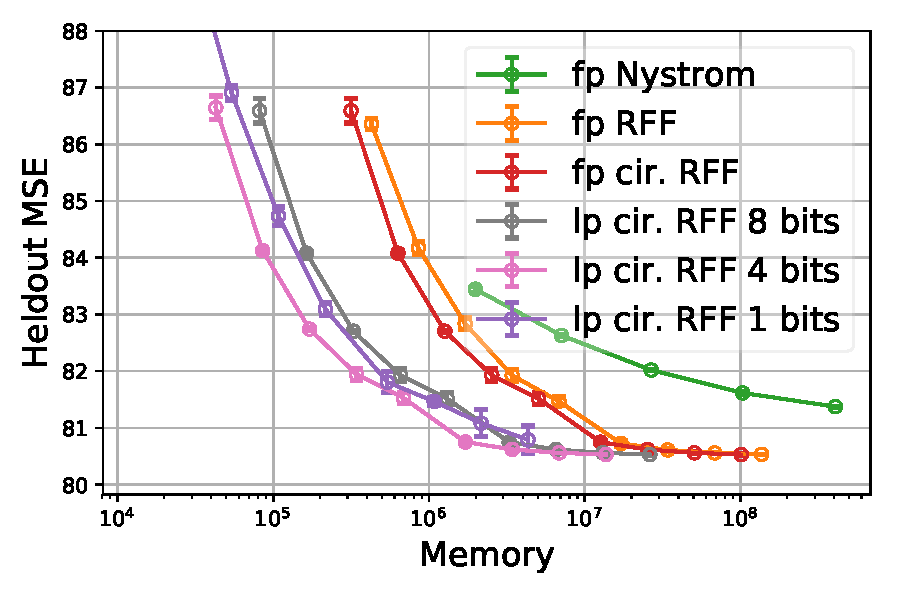
\includegraphics[width=0.3\linewidth]{figures/yearpred_MSE_vs_n_memory.pdf} &
%%		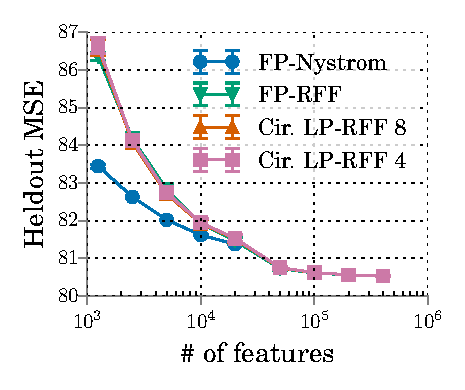
\includegraphics[width=0.3\linewidth]{figures/yearpred_MSE_vs_n_feat.pdf} &
%%		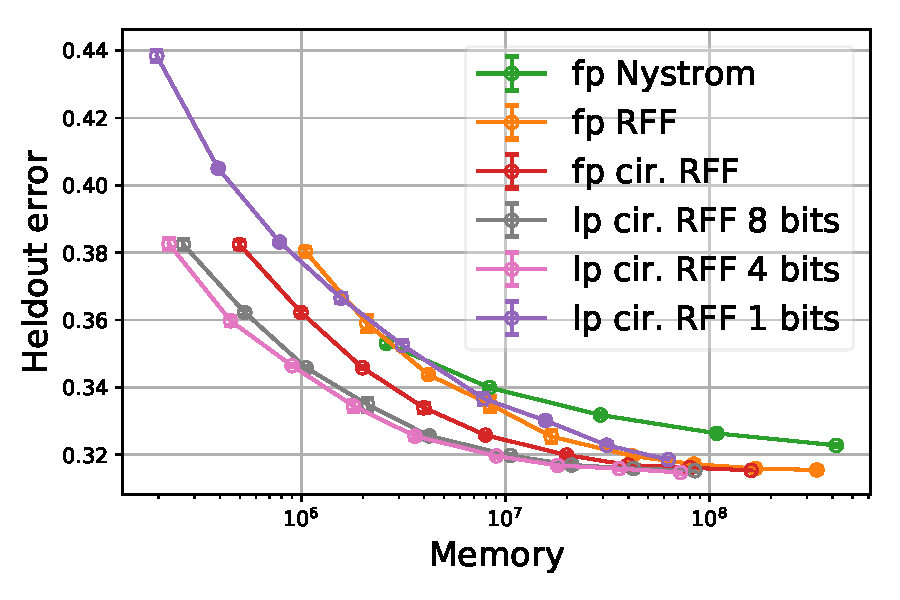
\includegraphics[width=0.3\linewidth]{figures/timit_error_vs_n_memory.pdf} &
%%		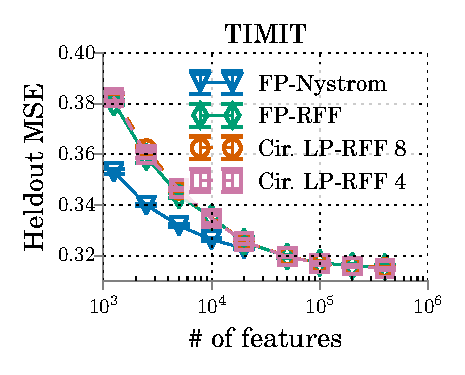
\includegraphics[width=0.3\linewidth]{figures/timit_error_vs_n_feat.pdf} \\
%%		(a) Census & (b) YearPred & (c) Covtype & (d) TIMIT \\
%%		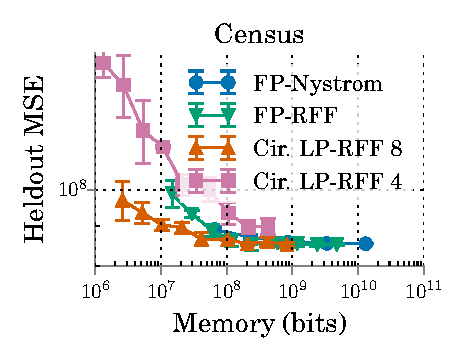
\includegraphics[width=0.3\linewidth]{figures/census_MSE_vs_n_memory.pdf} &
%%		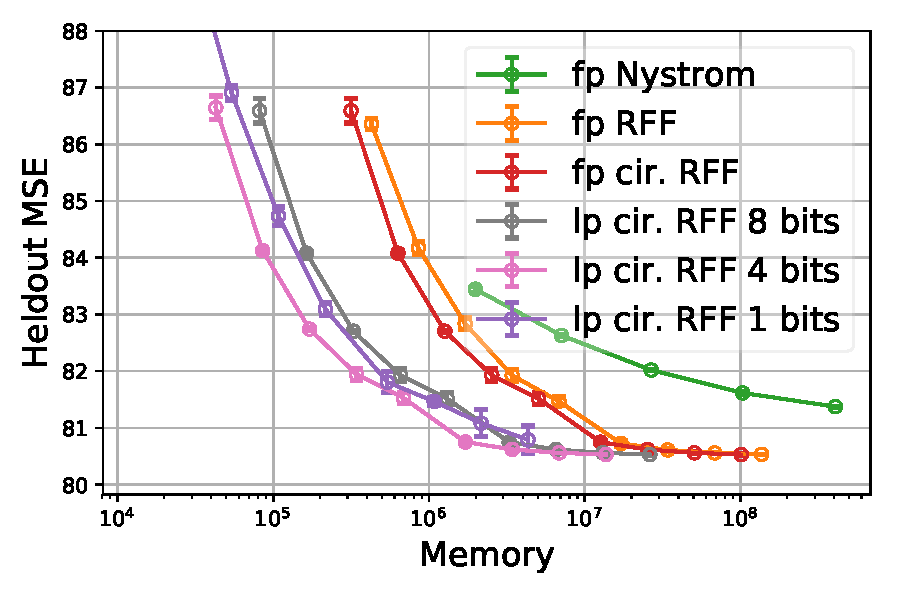
\includegraphics[width=0.3\linewidth]{figures/yearpred_MSE_vs_n_memory.pdf} &
%%		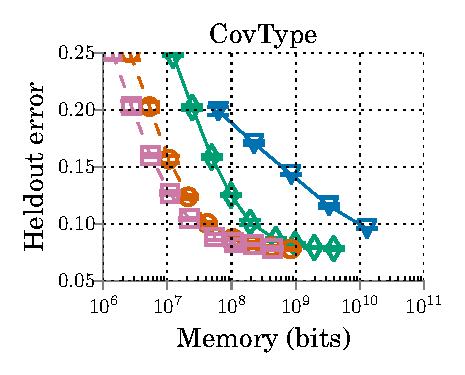
\includegraphics[width=0.3\linewidth]{figures/covtype_error_vs_n_memory.pdf} &
%%		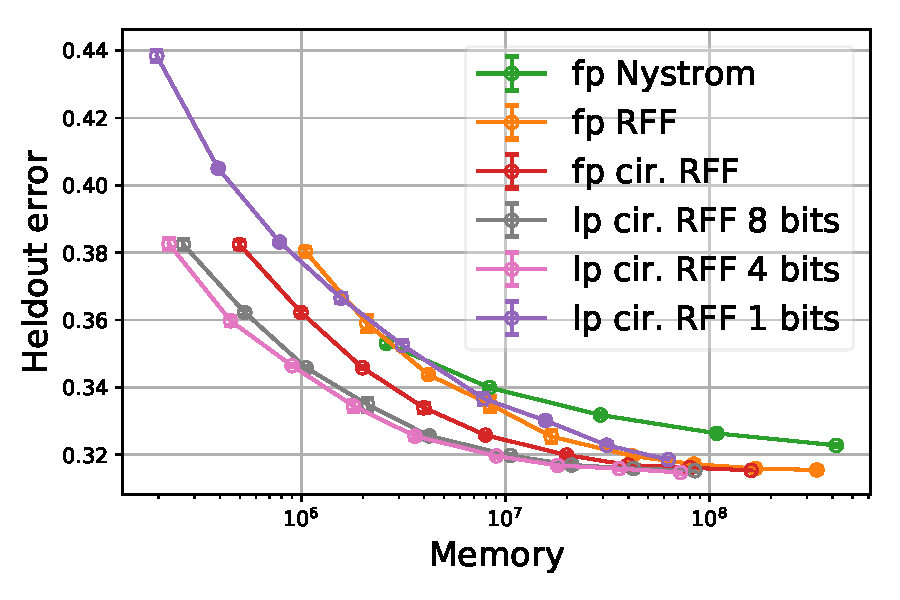
\includegraphics[width=0.3\linewidth]{figures/timit_error_vs_n_memory.pdf} \\
%%		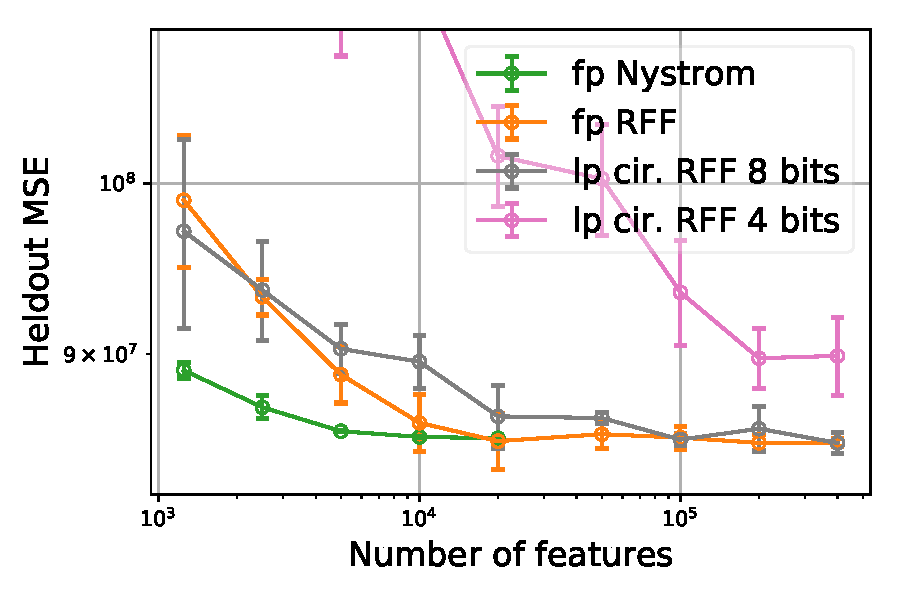
\includegraphics[width=0.3\linewidth]{figures/census_MSE_vs_n_feat.pdf} &
%%		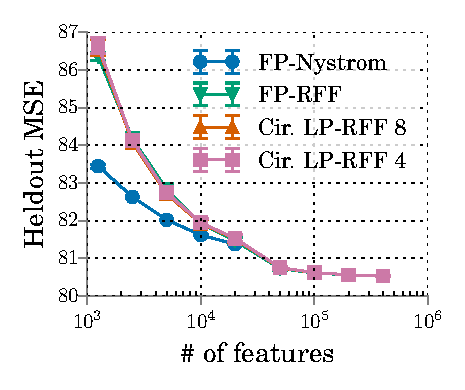
\includegraphics[width=0.3\linewidth]{figures/yearpred_MSE_vs_n_feat.pdf} &
%%		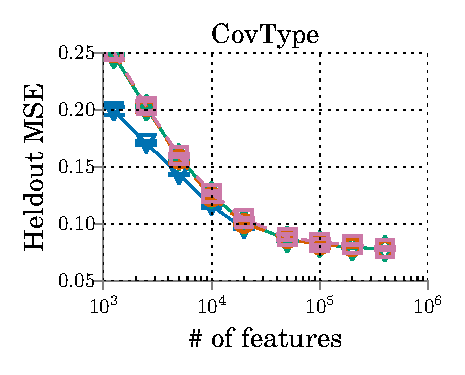
\includegraphics[width=0.3\linewidth]{figures/covtype_error_vs_n_feat.pdf} &
%%		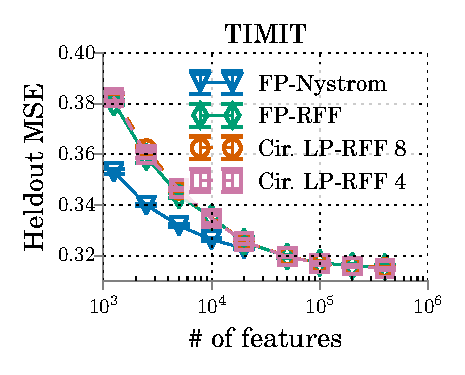
\includegraphics[width=0.3\linewidth]{figures/timit_error_vs_n_feat.pdf} \\
%%		(a) Census & (b) YearPred & (c) Covtype & (d) TIMIT \\
%	\end{tabular}
%	\end{small}
%	\caption{Generalization performance of LP-RFFs, FP-RFFs, and \Nystrom with respect to memory and number of features, on TIMIT and YearPred.  For CovType \& Census, see Appendix~\ref{subsec:app_exp_detail}.
%		%  LP-RFFs demonstrate better generalization performance than the full precision methods, under a memory budget. It is also informative to observe that while the \Nystrom method attains the best generalization performance with respect to the number of features, it is the worst performance method as a function of memory.  For results on the CovType and Census datasets, please see Figure~\ref{fig:generalization_col_app} in Appendix~\ref{sec:exp_details}
%}
%	\label{fig:generalization_col}
%\end{figure}

%% version with out model memory
%\begin{table}
%	\centering
%	\begin{tabular}{c c c c}
%		\hline
%		& FP RFF & FP circulant RFF & \Nystrom \\
%		\hline
%		\hline
%		Census & 5.56x & 30.32x & 122.52x \\
%		YearPred & 19.35x & 14.30x & 829.15x \\ 
%		Covtype & 9.17x & 7.57x & 460.80x \\ 
%		TIMIT & 70.42x & 25.68x & 843.41x \\ 
%		\hline
%	\end{tabular}
%	\caption{The memory savings from LP RFF to achieve within $1e^{-4}$ relative difference from the best generalization performance of baselines. We measure heldout L2 loss and heldout accuracy as the generalization performance respectively for regression and classification problems.}
%	\label{fig:mem_saving}
%\end{table}

% version with model memory
\begin{table}[ht]
\begin{minipage}{.57\linewidth}
\centering
%\vspace{0.42in}
	\begin{tabular}{c c c c}
		\toprule
		& FP-RFFs & Cir. FP-RFFs & \Nystrom \\
		\midrule
%		Census & 2.8x / 1.13x & 30.7x / 7.7x & 62.2x / 4.09x \\
%		YearPred & 10.0x / 7.3x & 14.7x / 10.8x & 436.9x / 78.0x \\ 
%		Covtype & 4.6x / 4.6x & 7.6x / 7.6x & 230.4x / 75.3x \\ 
%		TIMIT & 5.1x / 2.0x & 3.9x / 3.6x & 50.6x / 8.9x \\ 
%		Census & 2.9x / 1.15x & 15.6x / 3.9x & 63.2x / 4.2x \\
%		YearPred & 10.3x / 7.7x & 7.6x / 5.7x & 461.6x / 80.3x \\ 
%		Covtype & 4.7x / 4.7x & 3.9x / 3.9x & 237.2x / 77.5x \\ 
%		TIMIT & 5.1x / 2.0x & 2.4x / 2.2x & 50.9x / 8.9x \\ 
		Census & 2.9x & 15.6x & 63.2x \\
		YearPred & 10.3x & 7.6x & 461.6x \\ 
		Covtype & 4.7x & 3.9x & 237.2x \\ 
		TIMIT & 5.1x & 2.4x & 50.9x \\ 
		\bottomrule \\ \\
	\end{tabular}
	\caption{The compression ratios achieved by LP-RFF relative to the best performing configurations for each baseline (FP-RFFs, circulant FP-RFFs, \NystromNS).  %\todo{Put optimal \# bits in parentheses?}
		%For each baseline method, we find the best performing configuration as the reference performance, then record the memory consumption of the smallest LP-RFF and baseline models that are within $10^{-4}$ relative performance to this reference. The memory saving is reported as the ratio between the two recorded memory consumption.
	}
	\label{tab:mem_saving}
\end{minipage}
\hspace{0.15in}
\begin{minipage}{0.375\linewidth}
\vspace{-0.78em}
	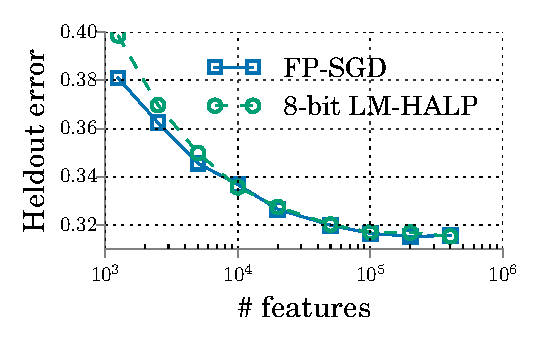
\includegraphics[width=0.975\linewidth]{figures/timit_error_vs_n_feat_lm_halp.pdf}
%	\caption{Low-precision training on TIMIT using 8-bit LM-HALP on 8-bit LP-RFFs, relative to full-precision SGD.
%		%Low precision training with HALP can demonstrate similar generalization performance as full precision training with SGD.
%	}	
	\caption{Low-precision 8-bit LM-HALP and full-precision SGD training on TIMIT using 8-bit LP-RFFs.}	
	\label{fig:halp}
\end{minipage}
\end{table}

%\label{sec:lptrain}
%\begin{figure}
%\centering
%	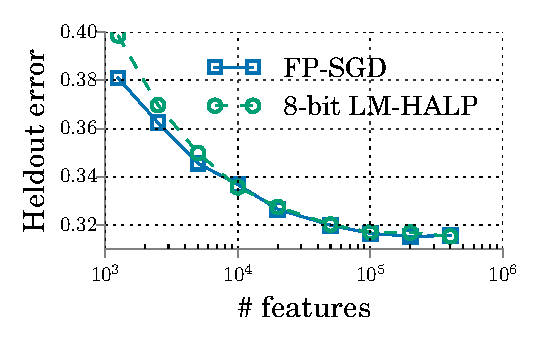
\includegraphics[width=.6\linewidth]{figures/timit_error_vs_n_feat_lm_halp.pdf}
%\label{fig:halp}
%\caption{Low precision training using HALP can demonstrate similar generalization performance as full precision training with SGD.}	
%\end{figure}
\vsp
\subsection{Generalization performance vs. relative spectral distance}
\label{subsec:perf_vs_rel_spec_dist}
We now aim to better understand the strong generalization performance of LP-RFFs, by seeing whether these results can be understood in terms of the theory presented in Sections \ref{sec:genbound} and \ref{sec:lprff}.  In particular, the theory we presented bounds the generalization performance of the kernel approximation models using the relative spectral distance between the kernel approximation matrix, and the exact kernel matrix.  Although the theory as presented only applies to fixed design linear regression, we empirically verify that relative spectral distance is predictive of generalization performance for non-fixed design kernel ridge regression, as well as for kernel logistic regression.

We run experiments on the Census dataset, as well as on a sub-sampled version of the CovType dataset, where we select $20k$ training and heldout points at random.  The reason we use these smaller datasets is because computing the relative spectral distance is an expensive operation, which requires instantiating the kernel matrices fully, and performing singular value decompositions. For the Census dataset, we use the closed form solution for the kernel ridge regression estimator.  For CovType, because there is no closed form solution for logistic regression, we train the models with SGD using mini-batches of size 250; we pick the best initial learning rate, as well as regularization parameter, by using $20k$ \Nystrom features as a proxy for the exact kernel (note that because there are only $20k$ training points, this \Nystrom approximation is exact). For CovType, we pick the initial learning rate from the set $\{5, 10, 50, 100\}$, and for both tasks we pick the regularization parameter $\lambda \in \{1e^{-5}, 5e^{-5}, 1e^{-4}, 1e^{-3}, 5e^{-3}, 1e^{-2}, 5e^{-2}, 1e^{-1}\}$ which gives the best performance on the heldout set. We report the average $D_{\lambda}(K,\tK)$ and the average generalization performance, along with standard deviations, using 5 different random seeds.

In Figure~\ref{fig:specdist} (left), we observe that LP-RFFs can achieve significantly smaller relative spectral distance $D_{\lambda}(K,\tK)$ than FP-RFFs and the \Nystrom method under a fixed memory budget. For example, the 8-bit LP-RFFs attain the best relative spectral distance for the Census dataset. This figure also shows generalization performance vs. relative spectral distance (middle), as well as vs.\ the Frobenius norm of $K-\tK$ (right). There is a strong correspondence between relative spectral distance and generalization performance across these methods, whereas for the Frobenius norm, the \Nystrom method does not align well with the RFF-based methods. The \Nystrom and RFF results also don't align well in terms of the spectral norm; see Appendix~\ref{subsec:app_additional_exp_res} for spectral norm results, as well as for results on CovType.

\begin{figure}
	\centering
%	\begin{tabular}{c c c}
%		\subfigure[MSE and relative spectral distance]{\label{fig:census_delta} 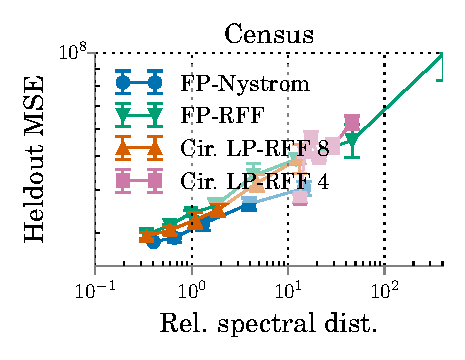
\includegraphics[width=0.33\linewidth]{figures/regression_l2_vs_delta.pdf} } \hfill
%		\subfigure[MSE and Frobenius norm]{\label{fig:census_f_norm} 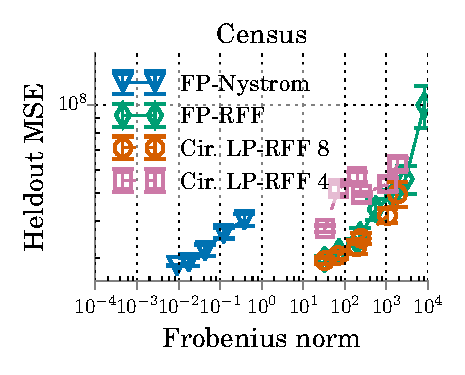
\includegraphics[width=0.33\linewidth]{figures/regression_l2_vs_f_norm.pdf} } \hfill
%		\subfigure[relative spectral distance and memory]{\label{fig:census_s_norm}  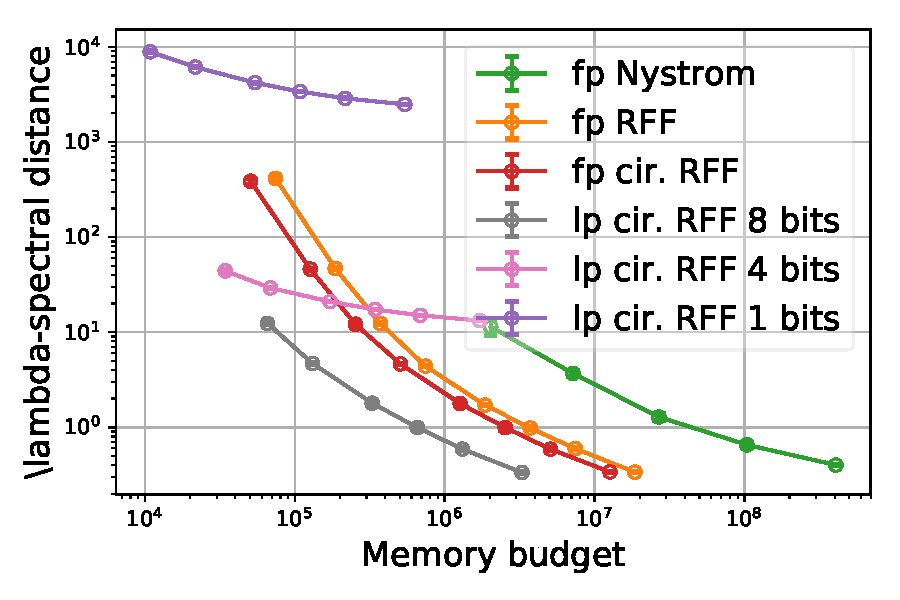
\includegraphics[width=0.33\linewidth]{figures/regression_delta_vs_mem.pdf} } \hfill \\
%		\subfigure[MSE and relative spectral distance]{\label{fig:covtype_delta} 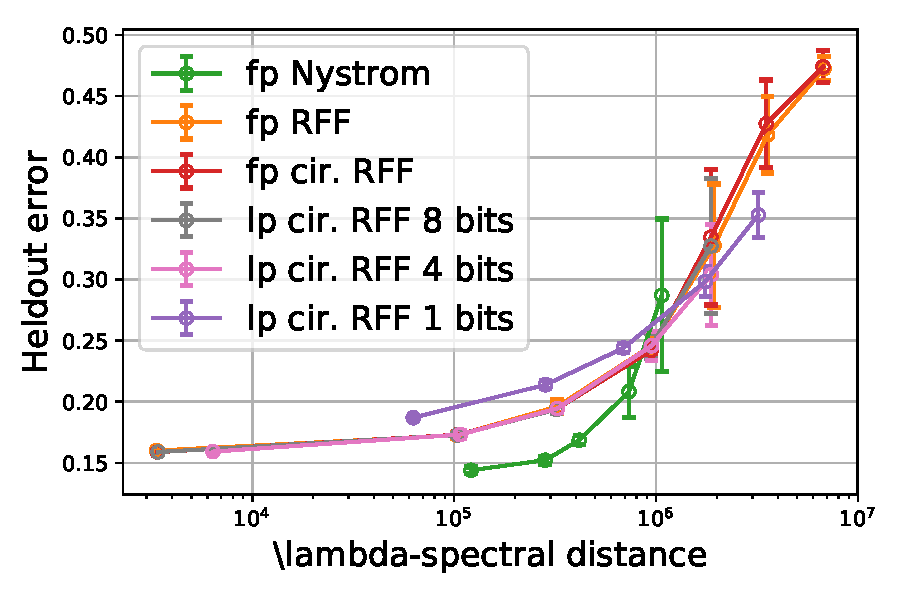
\includegraphics[width=0.33\linewidth]{figures/classification_acc_vs_delta.pdf} } \hfill
%		\subfigure[Error and Frobenius norm]{\label{fig:covtype_f_norm} 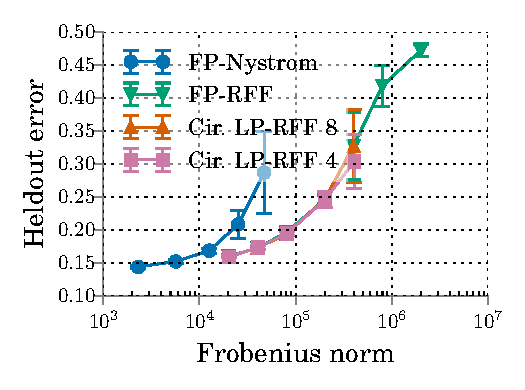
\includegraphics[width=0.33\linewidth]{figures/classification_acc_vs_f_norm.pdf} } \hfill
%		\subfigure[relative spectral distance and memory]{\label{fig:covtype_s_norm} \includegraphics[width=0.33\linewidth]{figures/classification_delta_vs_mem.pdf}} \hfill
%	\begin{tabular}{@{\hskip -0.1in}c@{\hskip -0.1in}c@{\hskip -0.1in}c@{\hskip -0.1in}}
%		\subfigure[Census: $D_{\lambda}(K,\tK)$ vs. memory]{\label{fig:census_s_norm}  \includegraphics[width=0.33\linewidth]{figures/regression_delta_vs_mem.pdf} } \hfill 
%		\subfigure[Census: MSE vs. $D_{\lambda}(K,\tK)$]{\label{fig:census_delta} \includegraphics[width=0.33\linewidth]{figures/regression_l2_vs_delta.pdf} } \hfill
%		\subfigure[Census: MSE vs. Frob. norm]{\label{fig:census_f_norm} \includegraphics[width=0.33\linewidth]{figures/regression_l2_vs_f_norm.pdf} } \hfill \\
%		\subfigure[CovType: $D_{\lambda}(K,\tK)$ vs. mem.]{\label{fig:covtype_s_norm} \includegraphics[width=0.33\linewidth]{figures/classification_delta_vs_mem.pdf}} \hfill
%		\subfigure[CovType: MSE vs. $D_{\lambda}(K,\tK)$]{\label{fig:covtype_delta} \includegraphics[width=0.33\linewidth]{figures/classification_acc_vs_delta.pdf} } \hfill
%		\subfigure[CovType: Error vs. Frob. norm]{\label{fig:covtype_f_norm} \includegraphics[width=0.33\linewidth]{figures/classification_acc_vs_f_norm.pdf} } \hfill
%	\end{tabular}
\begin{tabular}{@{\hskip -0.1in}c@{\hskip -0.1in}c@{\hskip -0.1in}c@{\hskip -0.1in}}
		\includegraphics[width=0.33\linewidth]{figures/regression_delta_vs_mem.pdf} &
		\includegraphics[width=0.33\linewidth]{figures/regression_l2_vs_delta.pdf} &
		\includegraphics[width=0.33\linewidth]{figures/regression_l2_vs_f_norm.pdf} %\vspace{-.1in}\\
%		\includegraphics[width=0.33\linewidth]{figures/classification_delta_vs_mem.pdf} &
%		\includegraphics[width=0.33\linewidth]{figures/classification_acc_vs_delta.pdf}&
%		\includegraphics[width=0.33\linewidth]{figures/classification_acc_vs_f_norm.pdf}
	\end{tabular}
	\caption{Analysis of generalization performance for Census, in terms of relative spectral distance $D_{\lambda}(K,\tK)$ and Frobenius norm $\frac{1}{n^2}\|K-\tK\|_F^2$. Comparing to Frobenius norm, relative spectral distance correlates stronger with generalization performance. For CovType, see Figure~\ref{fig:specdist_app} in Appendix~\ref{sec:exp_details}.
	%as a function of the memory utilization, and observe that LP-RFFs attain lower relative spectral distance per bit (rightmost plot). We then plot generalization performance as a function of relative spectral distance (middle), and Frobenius norm of $K - \tK$ (right). We observe a tigher correspondance between the generalization performance and relative spectral distance, relative to the Frobenius norm, on both datasets.
	}
	\label{fig:specdist}
\end{figure}

%\begin{figure}
%	\centering
%	\begin{tabular}{c c c}
%		\includegraphics[width=0.33\linewidth]{figures/regression_delta_vs_mem.pdf} &
%		\includegraphics[width=0.33\linewidth]{figures/regression_l2_vs_mem.pdf} &
%		\includegraphics[width=0.33\linewidth]{figures/regression_l2_vs_delta.pdf} \\
%		\includegraphics[width=0.33\linewidth]{figures/classification_delta_vs_mem.pdf} &
%		\includegraphics[width=0.33\linewidth]{figures/classification_acc_vs_mem.pdf} &
%		\includegraphics[width=0.33\linewidth]{figures/classification_acc_vs_delta.pdf} \\
%		(a) & (b) & (c)
%	\end{tabular}
%	\caption{The strong correlation between generalization performance and relative spectral distance $D_{\lambda}(K,\tK)$ under memory budgets for the Census dataset (top) and subsampled CovType dataset (bottom). Under different memory budget in (a) and (b), the precision demonstrates smaller $D_{\lambda}(K,\tK)$ tends to have better generalization performance. In (c), different kernel approximation approaches demonstrate similar generalization performance for similar relative spectral distance.}
%	\label{fig:specdist}
%\end{figure}
\vsp
\subsection{Low precision training for LP-RFFs}
\label{sec:halp}
Here, we show that we can train a model on top of LP-RFFs using low-precision model updates with a training algorithm called LM-HALP (linear model HALP) \citep{halp18}. LM-HALP is based on the stochastic variance-reduced gradient (SVRG) algorithm. In LM-HALP, all of the matrix multiplications involved in the stochastic model updates are done using low-precision integer operations; however, the periodic computation of the full gradient is calculated in full-precision (this is embarrassingly parallelizable). We present our results using 8-bit LM-HALP on top of 8-bit LP-RFFs, and comparing to full-precision SGD training, in Figure~\ref{fig:halp}. We show that when the number of features is at least $\num[group-separator={,}]{10000}$ the performance of 8-bit LM-HALP closely matches that of the full-precision training.  See Appendix \ref{subsec:app_exp_detail} for further details on these experiments. For future work, we plan to investigate training algorithms for LP-RFFs which are entirely low-precision.


